% Metódy inžinierskej práce

\documentclass[10pt,twoside,slovak,a4paper]{article}

\usepackage[slovak]{babel}
%\usepackage[T1]{fontenc}
\usepackage[IL2]{fontenc} % lepšia sadzba písmena Ľ než v T1
\usepackage[utf8]{inputenc}
\usepackage{graphicx}
\usepackage{url} % príkaz \url na formátovanie URL
\usepackage{hyperref} % odkazy v texte budú aktívne (pri niektorých triedach dokumentov spôsobuje posun textu)
\usepackage{graphicx}
\graphicspath{ {./obrazky/} }
\usepackage{cite}
%\usepackage{times}

\pagestyle{headings}

\title{Vyhľadávanie najlepšieho ťahu v šachu\thanks{Semestrálny projekt v predmete Metódy inžinierskej práce, ak. rok 2023/24, vedenie: Vladimír Mlynarovič}} % meno a priezvisko vyučujúceho na cvičeniach

\author{Martin Kubiš\\[2pt]
	{\small Slovenská technická univerzita v Bratislave}\\
	{\small Fakulta informatiky a informačných technológií}\\
	{\small \texttt{xkubis@stuba.sk}}
	}

\date{\small 5. november 2023} % upravte



\begin{document}

\maketitle

\begin{abstract}
Šach je strategická stolová hra, ktorá sa skladá z šachovnice o rozmeroch 8x8 a 6 typov figúrok vo dvoch farbách. Aj keď sa na prvý pohľad zdá ako jednoduchá hra, neprestáva trápiť mozgy hráčov jak začiatočníkov, tak profesionálov. Od 50. rokov 20 storočia, kedy sa vyvinul prvý šachový robot, sa vývoj nezastavil a počítače už sú na míle ďaleko pred ľudskými hráčmi. Cielom článku je priblíženie čitateľovi metódy a techniky šachových algoritmov, ich optimalizácia. Taktiež aj porovnanie medzi klasickými šachovými algoritmami a algoritmami obohatené o umelú inteligenciu a akým spôsobom vyhľadávajú najlepší možný ťah.
\ldots
\end{abstract}



\section{Úvod}

Hranie šachu si vyžaduje veľa zručností, strategické myslenie, plánovanie určitých ťahov, schopnosť predvídať a  byť nepredvídateľný. Aby sa hráči zlepšili, či už na profesionálnej alebo amatérskej úrovni, musia rozvíjať svoje zručnosti a znalosti o šachových algoritmoch a stratégiach, ktoré sú kľúčom k úspechu v tejto komplexnej hre.

V tomto článku sa zameriame na najdôležitejšie algoritmy ako sú minimax algoritmus s alfa-beta pruningom, monte carlo tree search algoritmus, alebo využitie deep learningu, neurálnych sietí a umelej inteligencie a aké sú stratégie na vyhľadanie čo najlepších možných ťahov na prekonanie súpera. a poukážeme na využitie týchto algoritmov v modernom šachovom svete. Ďalej sa budeme venovať technickým výzvam spojeným s vývojom šachových programov a ich schopnosťou hrať na úrovni šachových majstrov. 


\section{Minimax algoritmus} \label{minimax}
Minimax algoritmus je rozhodovací algoritmus používaný v hrách na určenie najlepšieho možného ťahu pre hráča v hre pre dvoch hráčov s nulovým súčtom, ako je napríklad šach, piškôrky alebo dáma. 

V hre s nulovým súčtom sú zisky jedného hráča presne vyvážené stratami druhého hráča, takže súčet ziskov a strát hráčov je vždy nula. 

\subsection{Princíp fungovania Minimax algoritmu} \label{principMinimax}
Minimax algoritmus funguje tak, že predpokladá, že obaja hráči budú hrať optimálne, a potom určí najlepší ťah pre hráča, ktorý práve robí ťah. Hráč 1 sa snaží žískať, čo najväčší počet bodov, zatial čo hráč 2 sa snaží získať čo najmenší počet bodov.

Robí to tak, že zvažuje všetky možné ťahy, ktoré by hráč mohol urobiť, a potom hodnotí každý z týchto ťahov simulovaním zvyšku hry za predpokladu, že súper urobí svoj najlepší možný ťah. Algoritmus potom vyberie ťah, ktorý vedie k najlepšiemu výsledku pre hráča, za predpokladu, že súper ako odpoveď urobí svoj najlepší možný ťah.\cite{Minimax}
\begin{figure}[h]
    \centering
    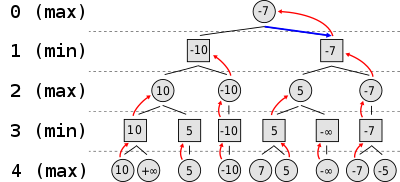
\includegraphics[width=\textwidth]{minimax}
    \caption{Jednoduchá ukážka minimax algoritmu}
    \label{obr1}
\end{figure}

\subsection{Výhody a obmedzenia Minimax algoritmu} \label {vyhodyMinimax}

Minimax algoritmus je výkonný rozhodovací algoritmus, ktorý poskytuje optimálne riešenia v zmysle teórie hier. Tento algoritmus má však niekoľko obmedzení. 

Prvým je jeho výpočtová náročnosť, najmä v hrách s veľkým rozhodovacím priestorom. Preto boli vyvinuté rôzne varianty a optimalizácie, ako napríklad:
\begin{itemize}
\item \nameref{alpha-beta}
\item Otváracie ťahy (Openings) \cite{ChessOpenings}
\end{itemize}
Vďaka týmto optimalizáciam sa zníži počet vetví, cez ktoré musí algoritmus prejsť, taktiež sa zlepší celkový výkon algoritmu. 

\section{Alpha-Beta pruning} \label{alpha-beta}
V praxi väčšina AI šachových robotov používa optimalizovanú verziu minimax algoritmu známeho ako alfa-beta pruning algoritmus. Základnou myšlienkou alfa-beta pruningu je zníženie počtu vetiev, ktoré je potrebné hodnotiť „prerezávaním“(pruningom) konárov, ktoré istotne nepovedú k lepšiemu výsledku ako tie, ktoré už boli hodnotené. 

To sa dosiahne použitím dvoch hodnôt, alfa a beta, na sledovanie najlepšieho výsledku, ktorý bol doteraz zistený pre maximalizujúceho hráča (alfa) a najlepšieho výsledku, ktorý bol doteraz nájdený pre minimalizujúceho hráča (beta).\cite{Alpha-Beta}

\subsection{Princíp fungovania alpha-beta pruningu} \label{principAlpha-beta}
Algoritmus funguje tak, že rekurzívne skúma strom hry a vyhodnocuje každý možný pohyb a výsledok pomocou algoritmu minimax. Pri skúmaní každej vetvy stromu aktualizuje hodnoty alfa a beta na základe najlepšieho výsledku, ktorý bol doteraz nájdený.

Ak nájde vetvu, v ktorej je výsledok pre minimalizujúceho hráča (beta) horší ako aktuálny najlepší výsledok pre maximalizujúceho hráča (alfa), prereže túto vetvu a prestane ju vyhodnocovať, pretože minimalizujúci hráč by tento ťah nikdy nezvolil. 

Algoritmus postupuje rekurzívne nahor po strome, pričom neustále aktualizuje hodnoty alfa a beta, kým nevyhodnotí všetky možné pohyby a výsledky, alebo kým neoreže všetky vetvy, ktoré sú zaručene horšie ako aktuálny najlepší výsledok.
\begin{figure}[h]
    \centering
    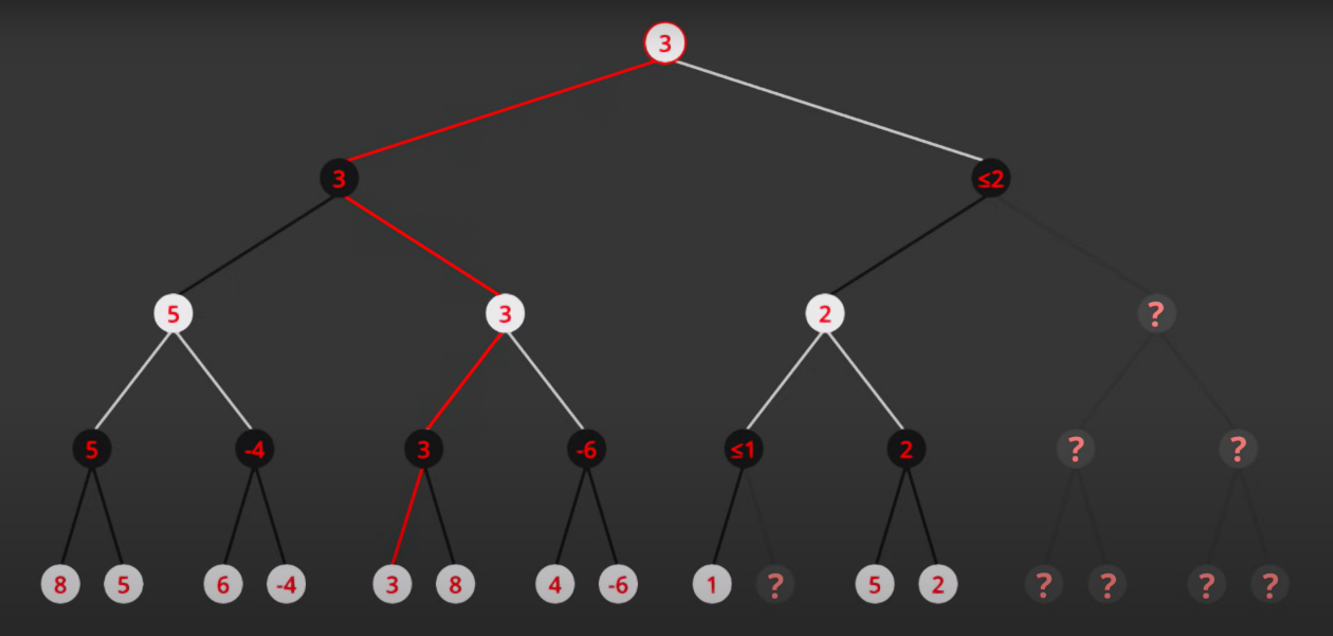
\includegraphics[width=\textwidth]{alpha-beta}
    \caption{ukážka alpha-beta pruningu}
    \label{obr2}
\end{figure}


\section{Monte Carlo Tree Search} \label{MonteCarlo}
Monte Carlo Tree Search (MCTS) je inovatívny a výkonný algoritmus v oblasti umelej inteligencie a teórie hier, ktorý bol využitý na rôzne stolové hry, ako je napríklad Go a šach. Tento algoritmus výrazne prekonáva tradičné techniky vyhľadávania v stromovom priestore, čím umožňuje získať vysokokvalitné výsledky v hrách s veľkými rozhodovacími priestormi.

\subsection{Princíp fungovania MCTS} \label{PrincipMTCS}
MCTS sa líši od predchádzajúcich algoritmov Minimax tým, že neprehľadáva celý stromový priestor. Namiesto toho sa používa metóda vzorkovania, pri ktorej sa ťahy vyberajú a simulujú až do konca hry, aby sa získal odhad aktuálneho stavu hry \cite{MCTS}. Opakuje tento proces niekoľkokrát a na základe získaných hodnôt sa rozhodne, ktorý ťah je najlepší. V MCTS existujú štyri základné fázy:
\begin{enumerate}
	\item výber (Selection)
	\item šírenie (Expansion)
	\item simulácia (Simulation)
	\item spätné šírenie (Backpropagation)
\end{enumerate}

\begin{figure}[h]
    \centering
    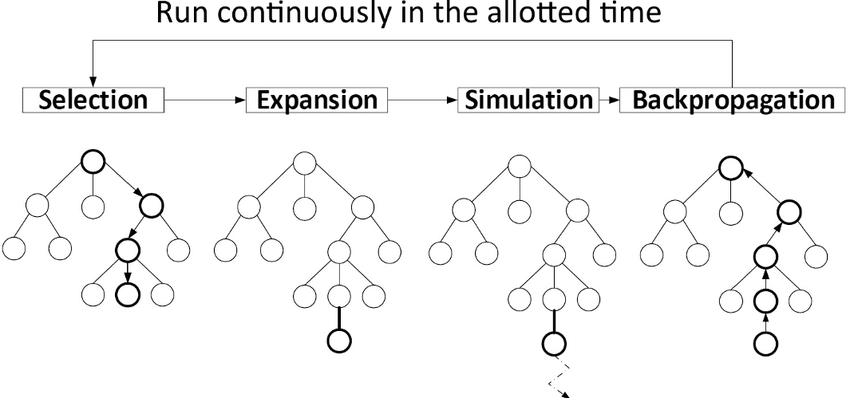
\includegraphics[width=\textwidth]{MCTS}
    \caption{ukážka fungovania MCTS}
    \label{obr3}
\end{figure}


\section{Umelá inteligencia a šach} \label{AI}

Význam umelej inteligencie pri hraní šachu je obrovský. Moderné šachové programy sú schopné hrať na úrovni a dokonca aj porážať majstrov sveta v šachu a stali sa cenným nástrojom pre hráčov všetkých úrovní. 

Umelá inteligencia umožňuje hráčom analyzovať svoje hry, trénovať, zlepšovať sa a objavovať nové stratégie. Vývoj v tejto oblasti pokračuje a umelá inteligencia bude hrať v budúcnosti šachu čoraz dôležitejšiu úlohu.
\subsection{Alpha zero} \label{alphaZeroAI}

Zlomovým bodom pre AI bolo predstavenie programu AlphaZero od DeepMind v roku 2017. \cite{AlphaZero} AlphaZero využíva kombináciu Deep Learningu a MCTS (\nameref{MonteCarlo}) na samoučenie hier. Program porazil najlepšie šachové programy na svete a dosiahol skvelé výsledky.

AlphaZero prináša nový pohľad na tréning umelej inteligencie, pretože sa učí šach bez ľudského tréningu alebo heuristiky, pričom dosahuje predtým nepredstaviteľnej úrovne. To znamená, že program sa neučil z predrom definovaných pravidiel, alebo ľudských stratégii, ale spoliehal sa na strojové učenie a analýzu veľkého množstva dát, ktoré sám generoval pri hraní šachu.

\subsection{význam AI v šachu} \label{RoleAI}
Umelá inteligencia prináša radu významých prínosov do sveta šachu
\begin{enumerate}
	\item výkon a sila

AI umožnuje vytvárať šachové programy, ktoré sú o dosť výkonnejšie, ako najlepší ľudskí hráči
	\item Samo-učenie

Pomocou AI sa šachové programy vedia učiť samé, čo znamená, že niesú obmedzené ľudskými znalosťami alebo stratégiami\cite{NeuralNetwork}. Napr. program AlphaZero, ako bolo už vyššie spomenuté.

	\item Analýza a tréning

Umelá inteligencia je už dnes bežne využívaná hráčmi na analýzu svojich hier, a na tréning. Šachové programy poháňané umelou inteligenciou sú skvelými učitelmi pre hráčov všetkých úrovní, keďže sa dokážu prispôsobovať svojim protivníkom.

\end{enumerate}

\section{Záver} \label{zaver} % prípadne iný variant názvu



%\acknowledgement{Ak niekomu chcete poďakovať\ldots}

\nocite{AlgorithmComparasion}
\nocite{AlgorithmComparasion2}
% týmto sa generuje zoznam literatúry z obsahu súboru literatura.bib podľa toho, na čo sa v článku odkazujete
\bibliography{literatura}
\bibliographystyle{plain} % prípadne alpha, abbrv alebo hociktorý iný
\end{document}
